\chapter{绘制轴承支座三视图}
{\bfseries 知识目标}
\begin{itemize}
\item 掌握三视图的形成规律
\item 掌握三视图的绘制方法
\item 掌握物体投影规律
\end{itemize}

{\bfseries 技能目标}
\begin{itemize}
\item 能够应用AutoCAD绘制零件的三视图
\item 能够应用三视图的投影规律完成零件的三视图
\end{itemize}

{\bfseries 本章导引}

本章我们将学习的重点是投影形成规律、三视图表达方法和物体投影规律。通过本章学习我们将具备将现实中的三维物体转换为符合国家规范的三视投影图的能力,并能够通过AutoCAD软件准确的绘制出来。图所示的项目是本章的最终任务,通过完成本章的一系列任务,我们将掌握三视图的绘制方法和步骤,具备一定的物体到视图的转换能力。

\noindent
\begin{figure}[htbp]
\centering
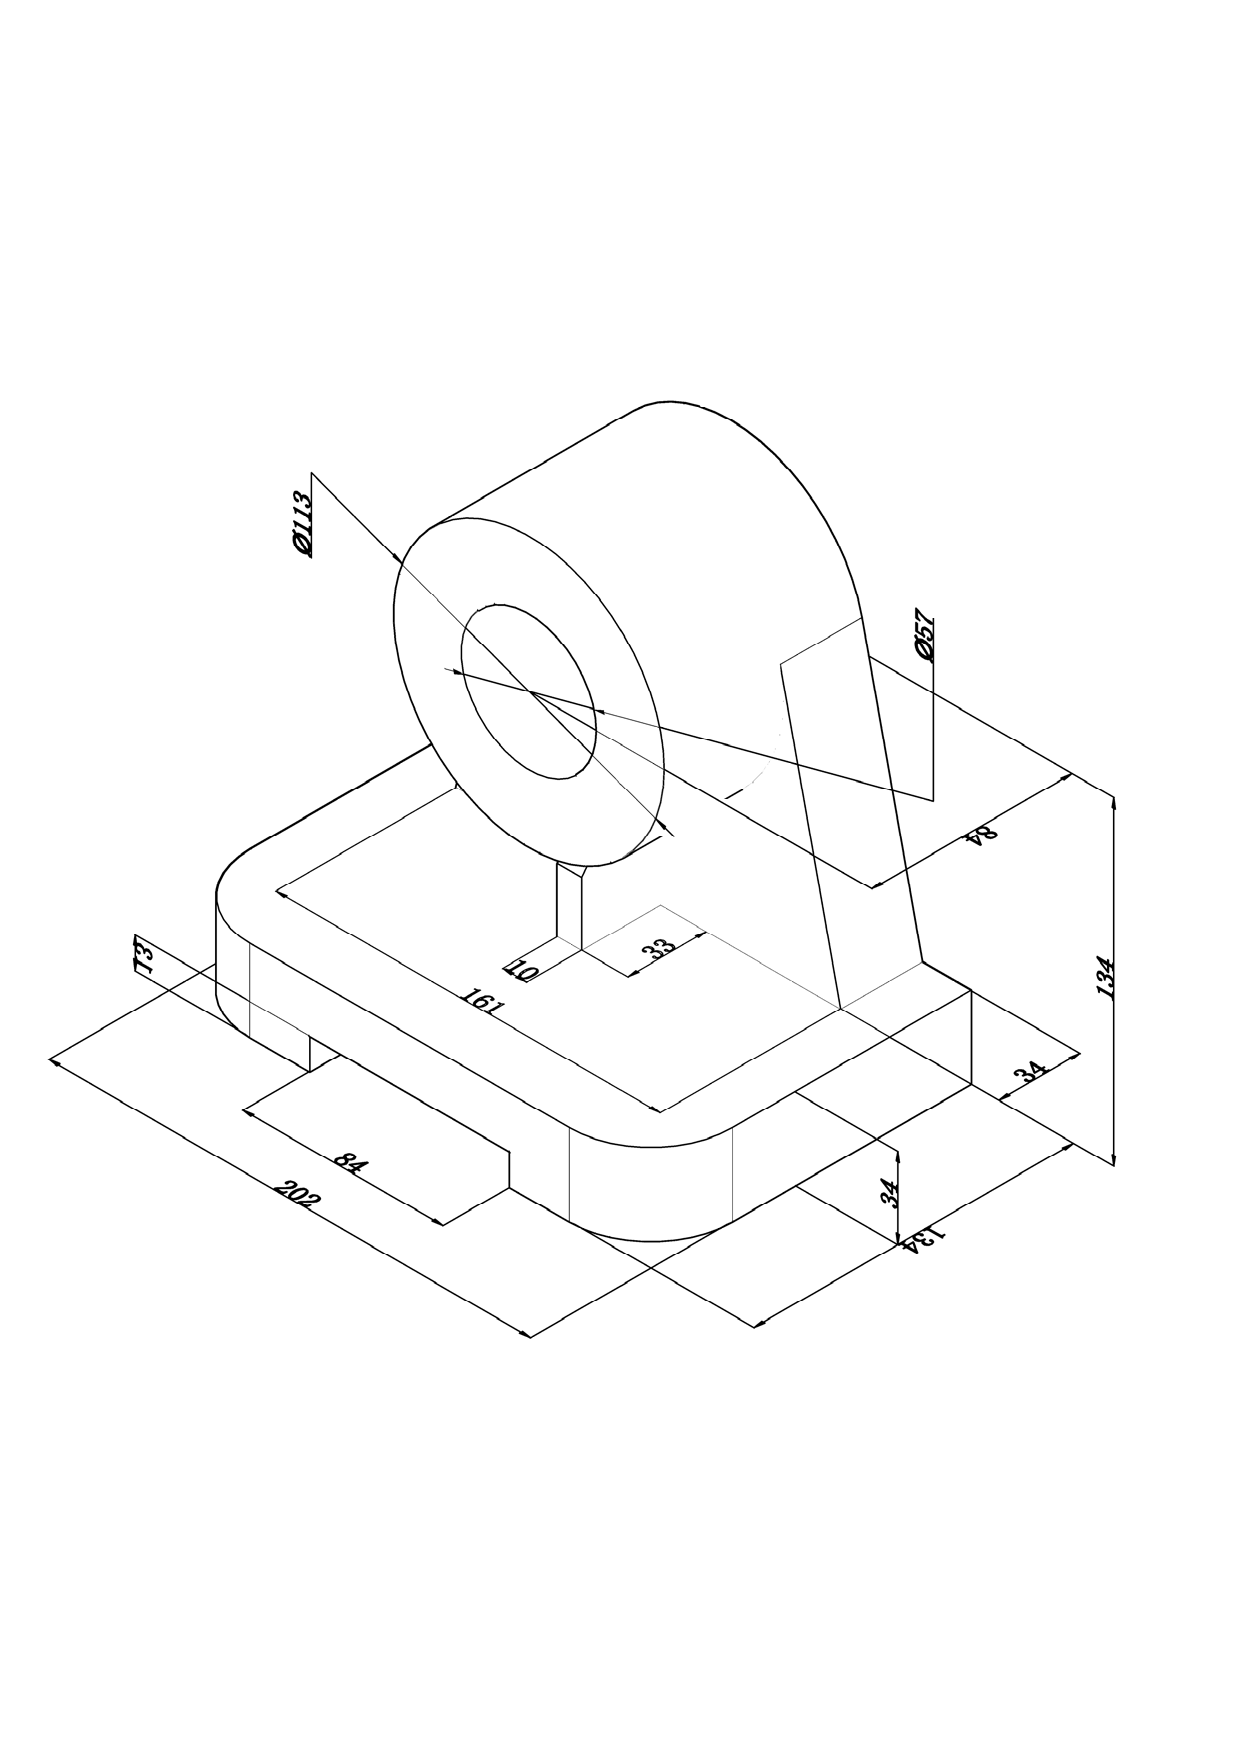
\includegraphics[scale=0.5]{zouchenzhizuo.pdf}
\caption{轴承支座}\label{fig:zouchenzhizuo}
\end{figure}

\endinput